\documentclass[12pt,a4paper]{article}

% ─── Packages ───────────────────────────────────────────────────────────────
\usepackage[margin=2.3cm]{geometry}
\usepackage{fontenc}
\usepackage{inputenc}
\usepackage{lmodern}
\usepackage{xcolor}
\usepackage{titlesec}
\usepackage{fancyhdr}
\usepackage{graphicx}
\usepackage{enumitem}
\usepackage{booktabs}
\usepackage{array}
\usepackage{tabularx}
\usepackage{longtable}
\usepackage{multirow}
\usepackage{hyperref}
\usepackage{tikz}
\usepackage{amsmath}
\usepackage{amssymb}
\usepackage{tcolorbox}
\usepackage{setspace}
\usepackage{parskip}
\usepackage{caption}
\usepackage{subcaption}
\usepackage{float}
\usepackage[normalem]{ulem}
\usepackage{adjustbox}
\usepackage{etoolbox}
\usepackage[nottoc]{tocbibind}

\usetikzlibrary{shapes.geometric, arrows, positioning, fit, backgrounds}

% ─── Color Palette ─────────────────────────────────────────────────────────
\definecolor{kintsuPink}{HTML}{E91E8C}
\definecolor{kintsuDark}{HTML}{1A1A2E}
\definecolor{kintsuGray}{HTML}{444444}
\definecolor{kintsuLight}{HTML}{FDE8EF}
\definecolor{kintsuteal}{HTML}{2DD4A8}
\definecolor{kintsugold}{HTML}{F5A623}
\definecolor{featurebox}{HTML}{FFF0F7}

% ─── Typography & Spacing ───────────────────────────────────────────────────
\setstretch{1.2}

% ─── Section Styling (Article Format) ───────────────────────────────────────
\titleformat{\section}
  {\normalfont\Large\bfseries\color{kintsuDark}}
  {\thesection}{1em}{}
\titleformat{\subsection}
  {\normalfont\large\bfseries\color{kintsuPink}}
  {\thesubsection}{1em}{}
\titleformat{\subsubsection}
  {\normalfont\normalsize\bfseries\color{kintsuGray}}
  {\thesubsubsection}{1em}{}

% ─── Header & Footer ────────────────────────────────────────────────────────
\pagestyle{fancy}
\fancyhf{}
\fancyhead[L]{\textcolor{kintsuPink}{\textbf{KINTSU Project Report}}}
\fancyhead[R]{\textcolor{kintsuGray}{\small Study Without Context Switching}}
\fancyfoot[C]{\textcolor{kintsuGray}{\thepage}}
\renewcommand{\headrulewidth}{0.5pt}
\renewcommand{\headrule}{\hbox to\headwidth{\color{kintsuPink}\leaders\hrule height \headrulewidth\hfill}}

% ─── Custom Callout Boxes ───────────────────────────────────────────────────
\newtcolorbox{featurebox}[2][]{
  colback=featurebox,
  colframe=kintsuPink,
  fonttitle=\bfseries\color{kintsuPink},
  title={#2},
  #1,
  arc=4pt,
  boxrule=1pt,
  left=8pt, right=8pt, top=6pt, bottom=6pt,
}

\newtcolorbox{insightbox}[1][]{
  colback=kintsuteal!10!white,
  colframe=kintsuteal,
  arc=4pt,
  boxrule=1pt,
  left=8pt, right=8pt, top=6pt, bottom=6pt,
  #1,
}

\newtcolorbox{techbox}[2][]{
  colback=white,
  colframe=kintsuDark,
  fonttitle=\bfseries\color{kintsuDark},
  title={#2},
  #1,
  arc=4pt,
  boxrule=1pt,
  left=8pt, right=8pt, top=6pt, bottom=6pt,
}

% ─── Metadata ───────────────────────────────────────────────────────────────
\hypersetup{
  colorlinks=true,
  linkcolor=kintsuPink,
  urlcolor=kintsuteal,
  citecolor=kintsuGray,
  pdftitle={Kintsu -- Project Report},
  pdfauthor={Pranav Agarwal},
  pdfsubject={Study Without Context Switching},
}

\begin{document}

% ─── Header Block ──────────────────────────────────────────────────────────
\begin{center}
  {\color{kintsuPink}\rule{\textwidth}{2pt}}\\[0.3cm]
  {\Huge\bfseries\color{kintsuDark} K \, I \, N \, T \, S \, U}\\[0.2cm]
  {\large\bfseries\color{kintsuPink} Comprehensive Technical \& Architectural Project Report}\\[0.1cm]
  {\small\color{kintsuGray}\textit{Study Without Context Switching --- An Integrated Web-Based Learning Workspace}}\\[0.2cm]
  {\small \textbf{Author:} Pranav Agarwal \quad|\quad \textbf{Stack:} HTML5, Vanilla CSS3, Vanilla JS, Node.js, Express, MongoDB, Gemini AI API}\\[0.2cm]
  {\color{kintsuPink}\rule{\textwidth}{2pt}}
\end{center}

\vspace{0.2cm}

\begin{insightbox}
\textbf{Executive Summary:} Kintsu is a browser-based all-in-one study workspace designed to eliminate the severe cognitive tax caused by context switching during online self-study. When students watch technical lectures on YouTube, write notes in Notion, run code in VS Code, and build revision flashcards on Anki, switching tabs repeatedly degrades memory retention and focus. Kintsu unifies embedded video playback, timestamp-synced rich notes, an in-browser multi-language code compiler, AI-driven automated flashcard generation, and a student interaction heatmap into a single seamless interface.
\end{insightbox}

\tableofcontents
\vspace{0.4cm}
\hrule
\vspace{0.4cm}

% ════════════════════════════════════════════════════════════════════════════
\section{Problem Statement \& Market Opportunity}
% ════════════════════════════════════════════════════════════════════════════

\subsection{The Cognitive Tax of Context Switching}
Modern online learning relies heavily on video platforms such as YouTube, Coursera, and MIT OpenCourseWare. However, the ecosystem around video learning remains completely fragmented:
\begin{enumerate}[leftmargin=1.5cm]
    \item \textbf{Tab Overload \& Distraction:} A student watching a coding tutorial must keep open YouTube, Google Docs/Notion, an IDE (VS Code), StackOverflow, and ChatGPT. Switching between 5--8 tabs every few minutes triggers context switching tax, breaking deep focus (flow state).
    \item \textbf{Unlinked Notes:} When writing notes in a external document, notes lack temporal connection to the lecture video. Reviewing notes later leaves the student guessing: \textit{"At what exact point in the 2-hour lecture was this concept explained?"}
    \item \textbf{Friction in Practice:} To test code shown in a video, the student must minimize the video, switch to their terminal or editor, set up files, and run code. This high friction leads most students to passively watch without executing code.
    \item \textbf{Manual Flashcard Creation Tax:} Active recall via flashcards is scientifically proven to improve long-term retention. Yet manually copying concepts into Anki or Quizlet takes hours, leading students to skip active recall altogether.
\end{enumerate}

\subsection{The Kintsu Solution}
Named after \textit{Kintsugi} (the Japanese art of repairing broken pottery with gold), **Kintsu** repairs the fragmented online learning experience. By stitching together video playback, notes, execution environment, active recall, and analytics onto one single screen, Kintsu allows students to study uninterrupted.

% ════════════════════════════════════════════════════════════════════════════
\section{Product Architecture \& Core Philosophy}
% ════════════════════════════════════════════════════════════════════════════

\subsection{Zero-Framework Frontend Philosophy}
Unlike heavy modern web applications built with React, Next.js, or Angular, Kintsu’s frontend is intentionally engineered with **Vanilla HTML5, Vanilla CSS3, and ES6+ JavaScript**.
\begin{itemize}[leftmargin=1.2cm]
    \item \textbf{Maximum Speed:} Zero bundler overhead, zero heavy `node_modules` downloads on the client, and instantaneous DOM rendering.
    \item \textbf{Low Latency UI:} Synchronizing video state, text selection, code output, and dynamic canvas rendering requires direct DOM manipulation without virtual DOM diffing penalties.
    \item \textbf{Educational Transparency:} Demonstrates complete mastery of core web standards (DOM APIs, Fetch API, HTML5 contenteditable, CSS Flexbox/Grid, CSS Custom Properties).
\end{itemize}

\subsection{Modular Architectural Layers}
Kintsu follows a strict three-tier architecture:
\begin{enumerate}[leftmargin=1.2cm]
    \item \textbf{Presentation Layer (Browser Client):} Handles user interactions, YouTube IFrame player synchronization, rich text editing, code output rendering, theme switching, and local storage state persistence.
    \item \textbf{Application Layer (Node.js + Express API):} Manages authentication, secure API key proxies (Gemini AI \& Piston Compiler), session metadata persistence, and interaction data aggregations.
    \item \textbf{Data \& Service Layer (MongoDB Atlas + External APIs):} Stores user credentials, notes, flashcard decks, and video interaction logs. Communicates with external execution sandboxes and Google Gemini LLMs.
\end{enumerate}

% ════════════════════════════════════════════════════════════════════════════
\section{Detailed 5-Page UI Walkthrough \& User Flow}
% ════════════════════════════════════════════════════════════════════════════

Kintsu's user interface is structured into 5 cohesive pages designed for effortless navigation and clear visual hierarchy.

\subsection{Page 1: Public Landing Page}
\begin{itemize}[leftmargin=1.2cm]
    \item \textbf{Navigation Bar:} Features the bold wordmark logo **KINTSU** with brand accent colors, navigation links (\textit{Features, How It Works, Pricing, FAQ}), Dark/Light theme toggle switch, and primary Call-To-Action (CTA) buttons (\textit{Sign In / Start Free}).
    \item \textbf{Hero Section:} Displays a high-impact headline: \textit{"Study Without Context Switching"}. The phrase \textit{"context switching"} is highlighted with a half-height pink background accent bar (`#E91E8C`) using CSS isolated pseudo-elements. Subtitle explains the product in simple terms.
    \item \textbf{Live Moving Ticker Strip:} A continuous, infinite-scrolling horizontal bar framed by top and bottom dark borders (`2px solid #1a1a1a`). Displays key features with pink bullet separators (\textit{Video Player • Live Code Compiler • AI Flashcards • Auto Timestamps • Pause Heatmap}).
    \item \textbf{Interactive Workspace Demo Preview:} Shows an embedded glassmorphism mock interface of the Kintsu 3-column study workspace, giving visitors an immediate visual understanding of the software before signing up.
    \item \textbf{Problem vs. Solution Comparison Grid:} Contrast cards showing the frustrating "Old Way" (10+ open tabs, context loss, manual Anki cards) versus the "Kintsu Way" (1 workspace, 1 click timestamps, auto AI flashcards).
    \item \textbf{FAQ Accordion \& CTA Section:} Expandable common questions with smooth slide animations and a final full-width invitation to join.
\end{itemize}

\subsection{Page 2: Authentication Page (Sign In / Sign Up)}
\begin{itemize}[leftmargin=1.2cm]
    \item \textbf{Split Visual Layout:} Left side displays branding graphics and a revolving testimonial quotes carousel; right side contains the clean authentication form card.
    \item \textbf{Dual Auth Options:} Supports traditional Email/Password authentication as well as one-click "Continue with Google" OAuth 2.0 integration.
    \item \textbf{Validation \& Security Feedback:} Client-side real-time regex validation for password strength and email formatting, accompanied by clear error toast notifications.
\end{itemize}

\subsection{Page 3: User Dashboard}
\begin{itemize}[leftmargin=1.2cm]
    \item \textbf{Header Welcome Banner:} Personalized greeting (\textit{"Welcome back, Pranav!"}) displaying active study stats (Total study hours, notes written, flashcards generated).
    \item \textbf{Session Management Grid:} Visual cards representing past study sessions. Each card displays the video thumbnail, title, last edited date, note word count, and quick-action buttons (\textit{Open Workspace, Delete, Export PDF}).
    \item \textbf{New Workspace Creation Launcher:} Prominent "+" modal trigger allowing users to input a new YouTube URL or select subject tags to instantly spawn a fresh workspace session.
\end{itemize}

\subsection{Page 4: All-in-One Study Workspace (Core Product Page)}
The main workspace adopts a dynamic 3-column responsive desktop layout:
\begin{enumerate}[leftmargin=1.2cm]
    \item \textbf{Left Panel --- Media \& Heatmap Player:}
    Contains the YouTube IFrame player with custom playback speed buttons (0.5x to 2.0x), 10-second skip buttons, and the interactive Pause/Rewind Heatmap Strip directly beneath the scrubber bar.
    \item \textbf{Center Panel --- Smart Notes Editor:}
    A full-featured rich text editing canvas supporting bold, italic, headings, bullet lists, code blocks, and a prominent pink **"Stamp Timestamp"** button that drops live video time triggers directly into the text.
    \item \textbf{Right Panel --- Dual Tool Dock (Compiler \& AI Flashcards):}
    \begin{itemize}
        \item \textit{Tab A (Code Compiler):} Language selector dropdown (JavaScript, Python, C++, Java, Go), code editor textarea with line numbers, "Run Code" execute button, and isolated terminal output screen.
        \item \textit{Tab B (AI Flashcard Generator):} One-click "Generate Deck from Notes" button, AI progress spinner, interactive 3D flip card viewer, and "Add to Flashcard Library" save action.
    \end{itemize}
\end{enumerate}

\subsection{Page 5: Flashcard Library \& Spaced Repetition Review Page}
\begin{itemize}[leftmargin=1.2cm]
    \item \textbf{Deck Directory:} Grid of all generated flashcard decks organized by subject tags and session origin.
    \item \textbf{Study Mode Interface:} Full-screen focus mode implementing the Leitner 5-box spaced repetition system. Users click to flip cards, marking their confidence level (\textit{Easy, Medium, Hard}), which schedules card re-appearance automatically.
\end{itemize}

% ════════════════════════════════════════════════════════════════════════════
\section{Comprehensive Specification of the 5 Core Features}
% ════════════════════════════════════════════════════════════════════════════

\subsection{Feature 1: Automatic Timestamp-Linked Note Taking}
\begin{featurebox}{Feature 1 --- Timestamp Synchronization}
\textbf{Logic \& Implementation Workflow:} 
\begin{enumerate}[leftmargin=1.2cm]
    \item When the student clicks the **"Stamp Timestamp"** button while taking notes, JavaScript queries the YouTube IFrame Player API instance for the exact current playback time in seconds.
    \item The raw seconds float value (e.g., `148.62`) is formatted into human-readable minutes and seconds string (e.g., `"2:28"`).
    \item Using the browser DOM `Selection` and `Range` APIs, an inline HTML button element is inserted directly at the student's cursor caret position inside the notes content area.
    \item An event listener is bound to the generated button. When clicked in the future, it commands the YouTube player to seek to `148.62` seconds instantly and resume playback.
\end{enumerate}
\end{featurebox}

\subsection{Feature 2: Smart Rich Text Editor with Client-Side PDF Export}
\begin{featurebox}{Feature 2 --- Editor \& PDF Export}
\textbf{Logic \& Implementation Workflow:} 
\begin{enumerate}[leftmargin=1.2cm]
    \item Built on top of an HTML5 `contenteditable` container enriched with custom formatting controls (headings, lists, quotes, inline code).
    \item Auto-saves note drafts to local storage every 5 seconds to prevent accidental data loss.
    \item **PDF Export Pipeline:** When the user clicks "Export PDF", client-side JavaScript clones the notes DOM node, injects print-optimized CSS styles (converting interactive timestamp buttons into clear clean labels), and processes the node through `html2pdf.js` / `html2canvas` to output a multi-page PDF document.
\end{enumerate}
\end{featurebox}

\subsection{Feature 3: Multi-Language Live Code Execution Sandbox}
\begin{featurebox}{Feature 3 --- Live Code Compiler}
\textbf{Logic \& Implementation Workflow:} 
\begin{enumerate}[leftmargin=1.2cm]
    \item Enables students to test code directly beside video tutorials without installing local runtimes or switching to VS Code.
    \item **Execution Pipeline:** 
    \begin{itemize}
        \item Student selects language (e.g., Python, C++, JS) and clicks "Run Code".
        \item Client sends a REST `POST` request to Kintsu’s Express backend `/api/compile` endpoint containing language string and code body.
        \item Express backend validates request payload and proxies it to the isolated **Piston Execution Engine API** (sandboxed Docker containers).
        \item Piston compiles and executes the code within strict memory (128MB) and time limits (3 seconds), returning `stdout` or `stderr`.
        \item Backend forwards clean JSON response back to browser; client renders colored terminal output on the UI.
    \end{itemize}
\end{enumerate}
\end{featurebox}

\subsection{Feature 4: AI-Driven Flashcard Generator (Powered by Gemini AI)}
\begin{featurebox}{Feature 4 --- Gemini AI Flashcards}
\textbf{Logic \& Implementation Workflow:} 
\begin{enumerate}[leftmargin=1.2cm]
    \item Eliminates the manual work of creating revision flashcards.
    \item **Generation Pipeline:**
    \begin{itemize}
        \item Student clicks "Generate AI Flashcards" in the workspace.
        \item Backend receives the raw HTML notes content, strips formatting tags, and constructs a structured system prompt for the **Google Gemini API**.
        \item System prompt instructs Gemini to act as an expert tutor, identify core concepts, definition pairs, and problem-solution pairs, and output strictly formatted JSON arrays: `[{ question, answer }]`.
        \item Server parses Gemini's JSON response, validates schema structure, saves the card deck to MongoDB, and returns cards to client.
        \item Client renders interactive 3D CSS flip cards with smooth perspective transformations.
    \end{itemize}
\end{enumerate}
\end{featurebox}

\subsection{Feature 5: Video Pause/Rewind Interaction Heatmap}
\begin{featurebox}{Feature 5 --- Revision Heatmap Analytics}
\textbf{Logic \& Implementation Workflow:} 
\begin{enumerate}[leftmargin=1.2cm]
    \item Identifies exact video segments where the student struggled by tracking playback control behaviors.
    \item **Analytics Pipeline:**
    \begin{itemize}
        \item JavaScript attaches listeners to YouTube player state changes (`PAUSED`, `SEEKING`).
        \item If a pause occurs or a backward seek (rewind > 5 seconds) is triggered, an event log `{ videoId, timestamp, action }` is dispatched asynchronously to `/api/heatmap`.
        \item Express saves event entries into MongoDB.
        \item On session reload, backend returns aggregated event density for 10-second video bins.
        \item Frontend calculates opacity and maps values onto a multi-segment CSS color strip (`#E91E8C` gradient) placed directly under the video player. Darker segments highlight high-difficulty topics requiring revision.
    \end{itemize}
\end{enumerate}
\end{featurebox}

% ════════════════════════════════════════════════════════════════════════════
\section{Technology Stack Specifications}
% ════════════════════════════════════════════════════════════════════════════

\begin{techbox}{Full Stack Architecture Breakdown}
\begin{tabularx}{\textwidth}{l l X}
\toprule
\textbf{Layer} & \textbf{Technology} & \textbf{Purpose \& Rationalization} \\
\midrule
\textbf{Frontend} & HTML5 & Semantic document structure and accessible forms \\
\textbf{Frontend} & Vanilla CSS3 & Custom styling, Flexbox/Grid, Dark Mode variables, Keyframes \\
\textbf{Frontend} & ES6+ JavaScript & DOM manipulation, Fetch REST calls, YouTube API handling \\
\textbf{Frontend} & html2pdf.js & Client-side HTML element to multi-page PDF generation \\
\midrule
\textbf{Backend} & Node.js (v22 LTS) & High-concurrency event-driven asynchronous JS runtime \\
\textbf{Backend} & Express.js (v4.x) & Lightweight RESTful API routing, middleware, and controller logic \\
\textbf{Backend} & Mongoose (v8.x) & Object Data Modeling (ODM) layer for MongoDB schema enforcement \\
\textbf{Backend} & CORS \& Dotenv & Cross-origin resource sharing security and env management \\
\midrule
\textbf{Database} & MongoDB Atlas & Cloud NoSQL document database for flexible JSON data storage \\
\midrule
\textbf{External APIs} & YouTube IFrame API & Embedded video player control, state hooks, timestamp seeking \\
\textbf{External APIs} & Piston API & Sandboxed multi-language code compilation execution engine \\
\textbf{External APIs} & Gemini AI SDK & LLM integration for intelligent flashcard synthesis \\
\bottomrule
\end{tabularx}
\end{techbox}

% ════════════════════════════════════════════════════════════════════════════
\section{System Architecture \& Data Flow}
% ════════════════════════════════════════════════════════════════════════════

\subsection{Architectural Data Flow Diagram}

\begin{center}
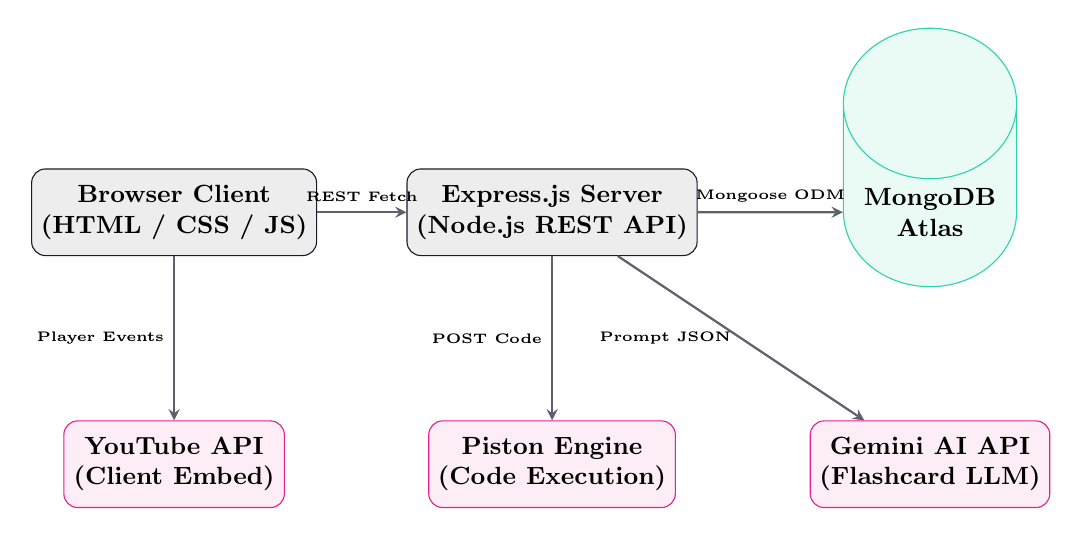
\begin{tikzpicture}[
  box/.style={rectangle, draw=kintsuDark, fill=kintsuDark!8, rounded corners=5pt, minimum width=2.8cm, minimum height=1.1cm, align=center, font=\small\bfseries},
  api/.style={rectangle, draw=kintsuPink, fill=kintsuPink!8, rounded corners=5pt, minimum width=2.8cm, minimum height=1.1cm, align=center, font=\small\bfseries},
  db/.style={cylinder, draw=kintsuteal, fill=kintsuteal!10, minimum width=2.2cm, minimum height=1.1cm, align=center, font=\small\bfseries, shape border rotate=90},
  arrow/.style={->, >=stealth, thick, draw=kintsuDark!70},
]
  % Nodes
  \node[box] (browser) at (0,0) {Browser Client\\\small(HTML / CSS / JS)};
  \node[box] (express) at (4.8,0) {Express.js Server\\\small(Node.js REST API)};
  \node[db] (mongo) at (9.6,0) {MongoDB\\\small Atlas};
  
  \node[api] (youtube) at (0,-3.2) {YouTube API\\\small(Client Embed)};
  \node[api] (piston) at (4.8,-3.2) {Piston Engine\\\small(Code Execution)};
  \node[api] (gemini) at (9.6,-3.2) {Gemini AI API\\\small(Flashcard LLM)};

  % Connections
  \draw[arrow] (browser) -- node[above, font=\tiny\bfseries]{REST Fetch} (express);
  \draw[arrow] (express) -- node[above, font=\tiny\bfseries]{Mongoose ODM} (mongo);
  
  \draw[arrow] (browser) -- node[left, font=\tiny\bfseries]{Player Events} (youtube);
  \draw[arrow] (express) -- node[left, font=\tiny\bfseries]{POST Code} (piston);
  \draw[arrow] (express) -- node[left, font=\tiny\bfseries]{Prompt JSON} (gemini);

\end{tikzpicture}
\end{center}

\subsection{Database Schema Design (Mongoose Models)}

The application utilizes 5 primary MongoDB collections:

\begin{enumerate}[leftmargin=1.2cm]
    \item \textbf{User Schema (`users`):} Stores `_id`, `name`, `email`, `passwordHash`, `googleId`, and `createdAt` timestamp.
    \item \textbf{Session Schema (`sessions`):} Stores `_id`, `userId` (ref: User), `videoUrl`, `videoId`, `videoTitle`, `subjectTag`, and `updatedAt`.
    \item \textbf{Note Schema (`notes`):} Stores `_id`, `sessionId` (ref: Session), `contentHTML` (rich text string with embedded timestamp triggers), `plainText`, and `lastSaved`.
    \item \textbf{Flashcard Deck Schema (`flashcards`):} Stores `_id`, `sessionId` (ref: Session), `userId` (ref: User), and `cards` array containing sub-documents: `[{ question, answer, confidenceScore, nextReviewDate }]`.
    \item \textbf{Heatmap Event Schema (`heatmapevents`):} Stores `_id`, `sessionId` (ref: Session), `videoId`, `timestampSeconds`, `actionType` (\textit{'pause'} or \textit{'rewind'}), and `loggedAt`.
\end{enumerate}

% ════════════════════════════════════════════════════════════════════════════
\section{CSS Design System \& Visual Aesthetics}
% ════════════════════════════════════════════════════════════════════════════

Kintsu enforces a modern design aesthetic engineered to feel premium:

\subsection{Color Palette \& Variables}
\begin{itemize}[leftmargin=1.2cm]
    \item \textbf{Primary Brand Accent:} `#E91E8C` (Kintsu Pink) --- Used for key interactive actions, active states, ticker highlights, and timestamp badges.
    \item \textbf{Dark Background Baseline:} `#1A1A2E` (Deep Midnight Dark) --- Prevents eye strain during long night study sessions.
    \item \textbf{Secondary Accents:} `#2DD4A8` (Teal for success/code outputs) and `#F5A623` (Warm Gold for flashcard indicators).
    \item \textbf{Light Mode Surface:} `#F9FAFB` with `#FFFFFF` cards and crisp `#111827` body text.
\end{itemize}

\subsection{Micro-Animations \& Visual Polish}
\begin{itemize}[leftmargin=1.2cm]
    \item \textbf{Glassmorphism Effects:} Panels utilize `backdrop-filter: blur(12px)` with subtle semi-transparent white border strokes (`rgba(255, 255, 255, 0.1)`).
    \item \textbf{Interactive Hover States:} Buttons feature scale shifts (`transform: translateY(-2px)`), glow shadows (`box-shadow: 0 4px 14px rgba(233, 30, 140, 0.4)`), and cubic-bezier transitions.
    \item \textbf{Ticker Animation:} Uses pure CSS `@keyframes ticker` executing continuous GPU-accelerated horizontal translation (`transform: translateX(-50%)`).
\end{itemize}

% ════════════════════════════════════════════════════════════════════════════
\section{Future Vision \& Roadmap}
% ════════════════════════════════════════════════════════════════════════════

\begin{enumerate}[leftmargin=1.2cm]
    \item \textbf{Version 1.0 (Current Baseline):} Single-video workspace, timestamp notes, live code compiler, Gemini AI flashcards, pause heatmap, dark mode, PDF export, landing page.
    \item \textbf{Version 2.0 (Planned Academic Update):} Multi-video course playlist support, peer-to-peer collaborative study rooms via WebSockets (shared notes + synchronized video playback), and Anki `.apkg` deck export file compatibility.
    \item \textbf{Version 3.0 (Long-Term AI Ecosystem):} Offline Progressive Web App (PWA) with background sync, voice-to-text live lecture transcription, and local WebLLM flashcard generation running fully client-side inside WebAssembly.
\end{enumerate}

% ════════════════════════════════════════════════════════════════════════════
\section{Project Conclusion}
% ════════════════════════════════════════════════════════════════════════════

\begin{center}
\begin{tcolorbox}[colback=featurebox, colframe=kintsuPink, arc=6pt, width=\textwidth, title={\bfseries\large Kintsu Project Summary in One Paragraph}]
\centering
\small
Kintsu successfully eliminates the context-switching penalty of modern web-based learning by integrating video playback, rich note-taking, live code compilation, AI flashcard synthesis, and behavioral analytics into a single high-performance workspace. Built upon clean web standards and scalable Node.js micro-services, Kintsu transforms passive video watching into an active, highly efficient, and deeply engaging learning experience.
\end{tcolorbox}
\end{center}

\vspace{0.4cm}
\begin{center}
  {\color{kintsuPink}\rule{8cm}{1pt}}\\[0.2cm]
  {\small\color{kintsuGray}\textit{End of Kintsu Technical Project Report}}
\end{center}

\end{document}
